\documentclass[12pt]{article}

\usepackage{algorithmic}
\usepackage{amsmath}
\usepackage{graphicx}
\usepackage{hyperref}
\usepackage{booktabs}

\begin{document}

\title{CSI709 Homework 4 \\
Gimp Bump Map Filter}
\author{
        Geoffrey Ulman \\
        George Mason University\\
}
\date{\today}

\maketitle

\section{Results}

My approach to replicate Gimp's \emph{Bump Filter} was to perform a simple shift and subtract gradient edge detection on a black and white version of the original image, then use the resulting detected edges to adjust the original color image. The image was lightened to one side of the edges and darkened on the other to create the illusion of light reflecting off bumps in the image.

\begin{figure}
\centering
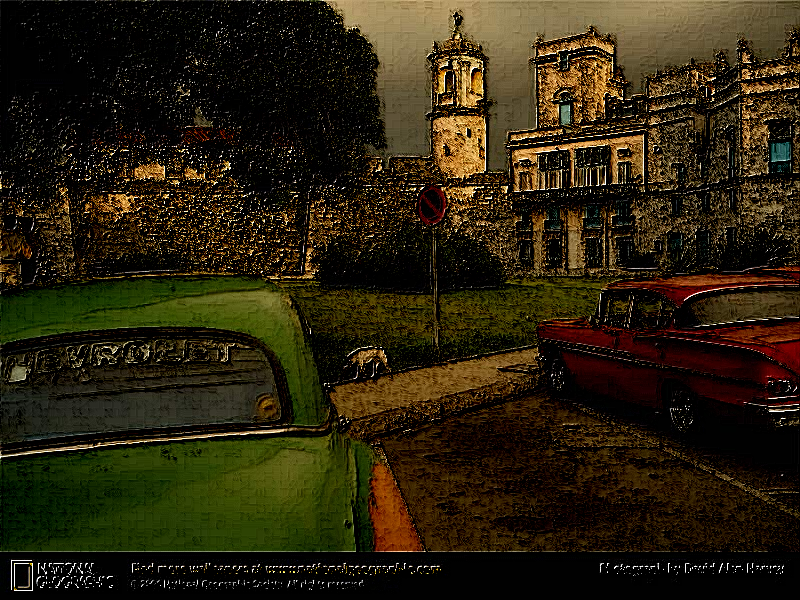
\includegraphics[width=1.00\textwidth]{geoff_ulman_homework4_result.png}
\caption{Result Image From My Algorithm}
\label{result_mine}
\end{figure}

\begin{figure}
\centering
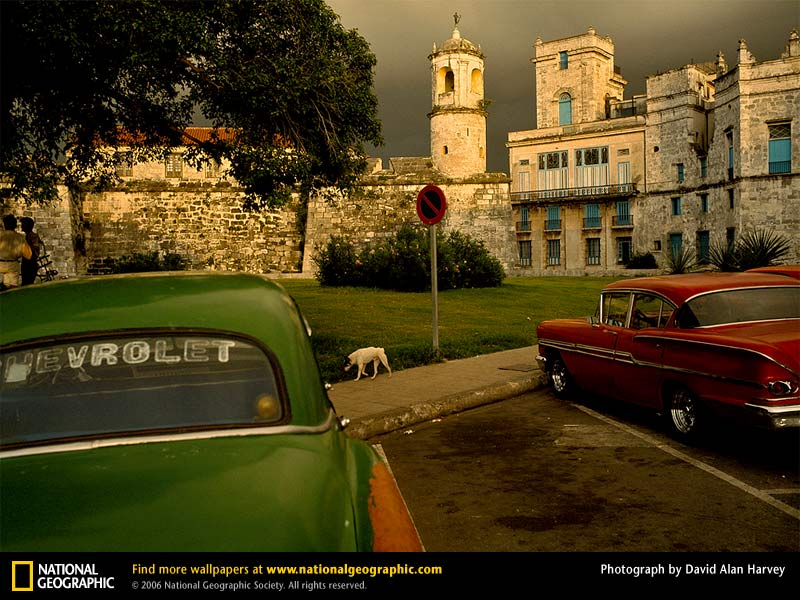
\includegraphics[width=1.00\textwidth]{car.png}
\caption{Input Image}
\label{original}
\end{figure}

\begin{figure}
\centering
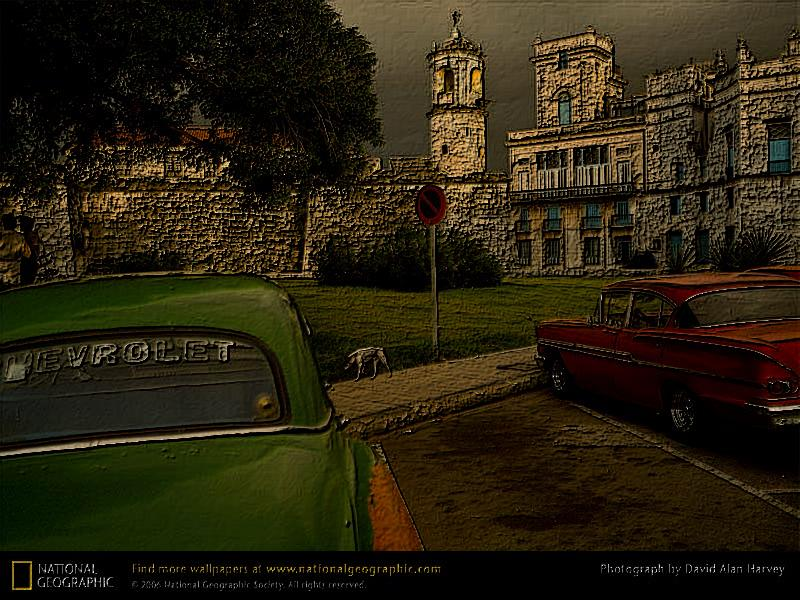
\includegraphics[width=1.00\textwidth]{car21.png}
\caption{Gimp Bump Filter Output}
\label{result_gimp}
\end{figure}


Figure \ref{result_mine} contains the output of my algorithm. For reference, Figure \ref{original} contains the unmodified image and Figure \ref{result_gimp} contains the output of Gimp's \emph{Bump Filter}.


\section{Formal Image Algebra}
Equation \ref{eq_edge} defines an edge finding function which highlights edges in a source image. The function \emph{edge} is then used in the bump mapping function described in Equation \ref{eq_bump} where three offset and scaled \emph{edge} functions are added to the original image.

\begin{figure}
\begin{equation}\label{eq_edge}
\begin{aligned}
\left\{ \left( \vec{x}, \textbf{edge}(\vec{x}) \right) : \textbf{edge}(\vec{x}) = \right. & \left. | \textbf{a}(\vec{x}+(1,1)) - \textbf{a}(\vec{x}) |, \vec{x} \in  \textbf{X} \right\}
\end{aligned}
\end{equation}
\caption{Edge Detection Helper Function}
\end{figure}

\begin{figure}
\begin{equation}\label{eq_bump}
\begin{aligned}
\left\{ \left( \vec{x}, \textbf{bump}(\vec{x}) \right) : \right. & \\
\left. \textbf{bump}(\vec{x}) = \right. & \left. 4 \times \textbf{edge}(\vec{x}) + \right. \\
& \left. 3 \times \textbf{edge}(\vec{x}+(1,1)) + \right. \\
& \left. -1 \times \textbf{edge}(\vec{x}+(-1,-1)) + \textbf{a}(\vec{x}) , \vec{x} \in  \textbf{X} \right\}
\end{aligned}
\end{equation}
\caption{Bump Map Formal Description}
\end{figure}

\end{document}
